\documentclass{beamer}

\usepackage{soul}


\usetheme{Boadilla} 		

\setbeamersize{text margin left=1cm,text margin right=1cm}

% DEFINITON FOOTLINE
% here: empty
\setbeamertemplate{footline}
{%
\begin{beamercolorbox}{}
\end{beamercolorbox}%
}


\usepackage[english]{babel}
\usepackage[latin1]{inputenc}
\usepackage{color}
\usepackage{graphicx}
\graphicspath{{img/}}
\usepackage{setspace}	
%\usepackage[pdftex]{graphicx}

%TABELLEN
\usepackage{array}
%\usepackage{ctable}		%Tabellen mit Fu�oten
\usepackage{multirow}
\usepackage{booktabs}
	% Neue Tabellenbefehle in der array Umgebung
	\renewcommand{\arraystretch}{1.2} % Zeilenabstand
	\newcolumntype{C}[1]{>{\centering\let\\\tabularnewline}p{#1}}
	\newcolumntype{R}[1]{>{\raggedleft\let\\\tabularnewline}p{#1}}
	\newcolumntype{L}[1]{>{\raggedright\let\\\tabularnewline}p{#1}}

\setbeamercovered{transparent}


\title{Reglas de Asociaci\'on y An\'alisis de Canastas de Mercado}
\author{Jorge Gallego}
\institute{Inter-American Development Bank}
	
\date{2026}

\begin{document}

%%%%%%%%%%%%%%%%%%%%%%%%%%%%%%%%%%%%%%%%%%%%%%%
\frame{\titlepage}
%%%%%%%%%%%%%%%%%%%%%%%%%%%%%%%%%%%%%%%%%%%%%%%

\frame{
  \frametitle{Introducci\'on}


\begin{itemize}
\item  Los supermercados son estrat\'egicos al organizar sus productos\vspace{0.3cm}

\item Pocos detalles son dejados al azar\vspace{0.3cm}

\item Se agrupan para maximizar la probabilidad de compras conjuntas\vspace{0.3cm}

\item Los algoritmos de aprendizaje no supervisado han sido clave para esto\vspace{0.3cm}

\item Y no solo los supermercados lo hacen



\end{itemize}

}

%%%%%%%%%%%%%%%%%%%%%%%%%%%%%%%%%%%%%%%%%%%%%%%

\frame{
  \frametitle{Sistemas de Recomendaci\'on}


Los supermercados ubican los productos para inducir compras conjuntas.

}

%%%%%%%%%%%%%%%%%%%%%%%%%%%%%%%%%%%%%%%%%%%%%%%

\frame{
  \frametitle{Sistemas de Recomendaci\'on}


\begin{figure}\caption{Vintage}
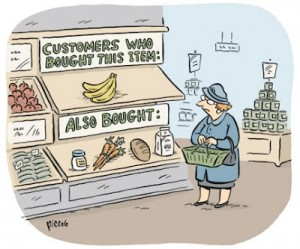
\includegraphics[scale=0.5]{vintage.jpg}
\end{figure}

}

%%%%%%%%%%%%%%%%%%%%%%%%%%%%%%%%%%%%%%%%%%%%%%%

\frame{
  \frametitle{Sistemas de Recomendaci\'on}


\begin{figure}\caption{Amazon}
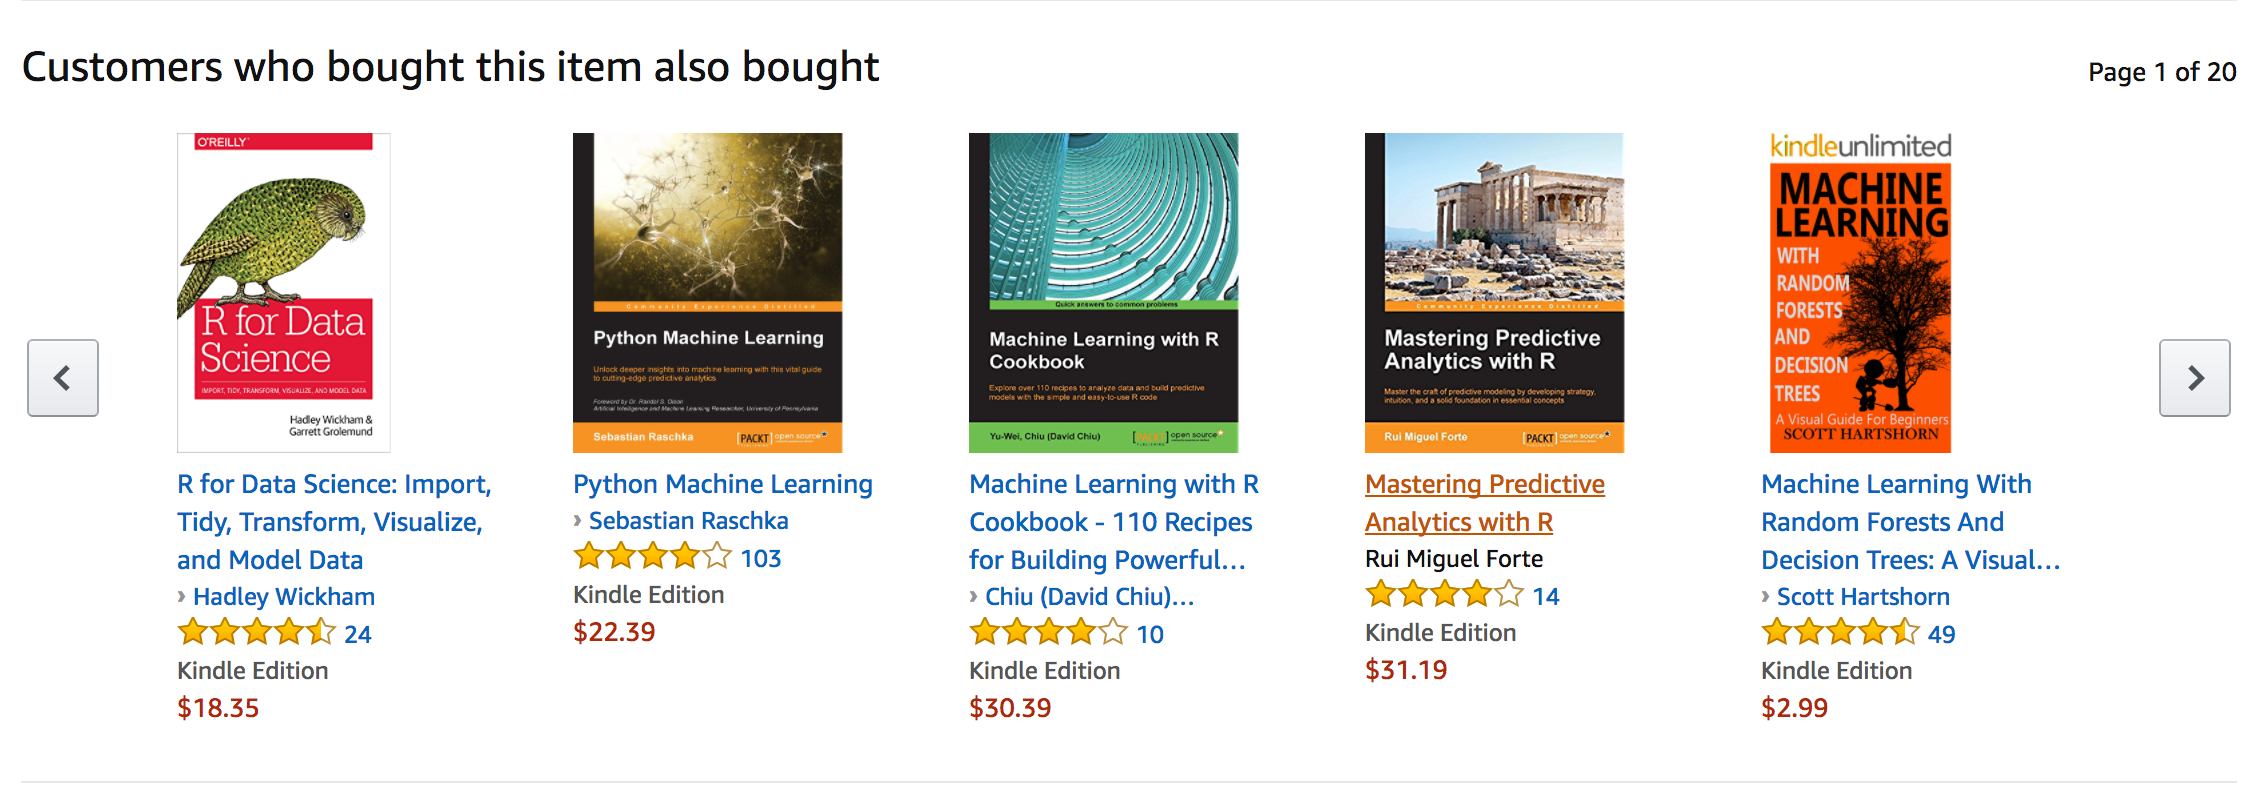
\includegraphics[scale=0.135]{amazon.png}
\end{figure}

}

%%%%%%%%%%%%%%%%%%%%%%%%%%%%%%%%%%%%%%%%%%%%%%%

\frame{
  \frametitle{Sistemas de Recomendaci\'on}


\begin{figure}\caption{Netflix}
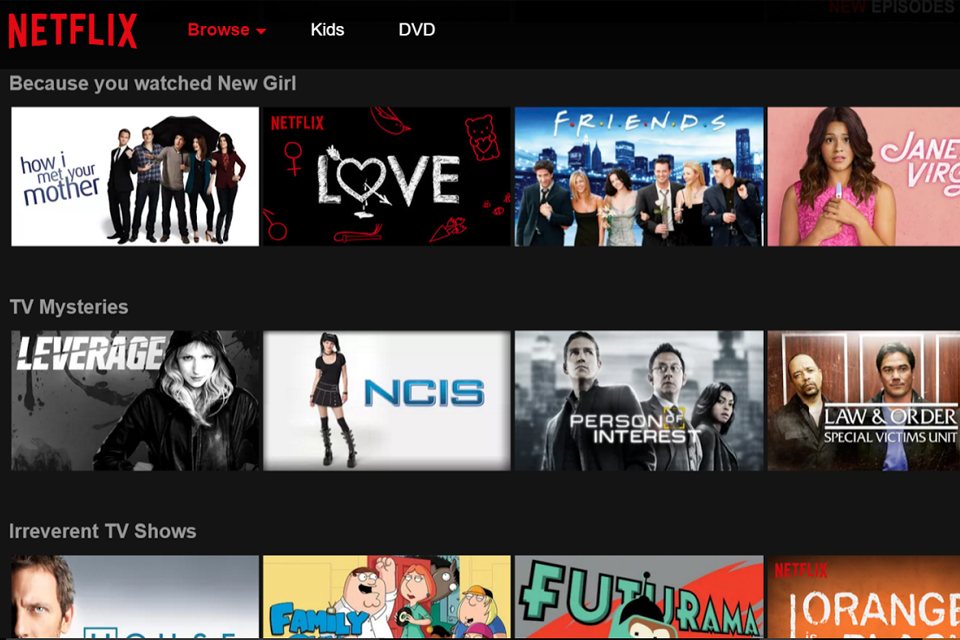
\includegraphics[scale=0.3]{netflix.jpg}
\end{figure}

}

%%%%%%%%%%%%%%%%%%%%%%%%%%%%%%%%%%%%%%%%%%%%%%%


\frame{
  \frametitle{Introducci\'on}


\begin{itemize}
\item  Por mucho tiempo estos sistemas se basaron en la intuci\'on de los vendedores\vspace{0.3cm}

\item Pero los datos disponibles hoy han revolucionado el tema \vspace{0.3cm}

\item Scanners de c\'odigos, sistemas digitales de inventario, compras en l\'inea, datos transaccionales \vspace{0.3cm}

\item T\'ecnicas de machine learning usan estos datos para encontrar patrones \vspace{0.3cm}

\item Veremos los fundamentos del \textit{market basket analysis} \vspace{0.3cm}


\end{itemize}

}

%%%%%%%%%%%%%%%%%%%%%%%%%%%%%%%%%%%%%%%%%%%%%%%

\frame{
  \frametitle{Reglas de Asociaci\'on}


\begin{itemize}
\item  El fundamento del an\'alisis son los items que forman parte de una transacci\'on\vspace{0.3cm}

\item Llamaremos \textbf{itemset} a un grupo de uno o varios items \vspace{0.3cm}

\item Por ejemplo: $\{\text{pan, jam\'on, queso}\}$ \vspace{0.3cm}

\item Construiremos reglas de asociaci\'on \vspace{0.3cm}

\item Especifican patrones encontrados en las relaciones entre items de un itemset \vspace{0.3cm}

\item Relacionan un itemset en el lado izquierdo de la relaci\'on, con otro en el lado derecho



\end{itemize}

}

%%%%%%%%%%%%%%%%%%%%%%%%%%%%%%%%%%%%%%%%%%%%%%%

\frame{
  \frametitle{Reglas de Asociaci\'on}


\begin{itemize}
\item  Una regla de asociaci\'on puede ser:

\[
\{\text{jam\'on, queso}\} \rightarrow \{\text{pan}\}
\]
\vspace{0.1cm}

\item Significa que si se compra jam\'on y queso, es  probable que se compre pan tambi\'en\vspace{0.3cm}

\item Ac\'a el objetivo central no es predecir sino encontrar patrones interesantes de manera no supervisada  \vspace{0.3cm}

\item No es necesario entrenar un modelo como tal, ni identificado en una categor\'ia u otra  \vspace{0.3cm}



\end{itemize}

}

%%%%%%%%%%%%%%%%%%%%%%%%%%%%%%%%%%%%%%%%%%%%%%%

\frame{
  \frametitle{Algoritmo Apriori}


\begin{itemize}
\item  Incluso para las m\'aquinas es complejo analizar datos transaccionales\vspace{0.3cm}

\item Suelen ser bases de datos muy grandes\vspace{0.3cm}

\item Muchas transacciones y muchos productores transados \vspace{0.3cm}

\item El n\'umero de itemsets crece exponencialmente\vspace{0.3cm}

\item Es imposible evaluarlos a todos para encontrar patrones


\end{itemize}

}

%%%%%%%%%%%%%%%%%%%%%%%%%%%%%%%%%%%%%%%%%%%%%%%

\frame{
  \frametitle{Algoritmo Apriori}


\begin{itemize}
\item  Para hacer el proceso m\'as eficiente se descartan itemsets\vspace{0.3cm}

\item Aquellos poco frecuentes, de baja probabilidad\vspace{0.3cm}

\item Por ejemplo: $\{\text{aceite de motor, labial}\}$\vspace{0.3cm}

\item Las combinaciones raras y poco importantes son ignoradas\vspace{0.3cm}

\item Esto es importante para disminuir el n\'umero de asociaciones posibles



\end{itemize}

}

%%%%%%%%%%%%%%%%%%%%%%%%%%%%%%%%%%%%%%%%%%%%%%%

\frame{
  \frametitle{Algoritmo Apriori}


\begin{itemize}
\item  El algoritmo m\'as usado para reducir el n\'umero de itemsets es el Apriori\vspace{0.3cm}

\item Se utilizan creencias simples sobre la frecuencia de un itemset \vspace{0.3cm}

\item Supuesto: un itemset es frecuente si sus subconjuntos son frecuentes tambi\'en\vspace{0.3cm}

\item $\{\text{aceite de motor, labial}\}$ son frecuentes si $\{\text{aceite de motor}\}$ y $\{\text{labial}\}$ son frecuentes tambi\'en \vspace{0.3cm}

\item Si alguno de los dos es infrecuente, el itemset conjunto lo ser\'a




\end{itemize}

}

%%%%%%%%%%%%%%%%%%%%%%%%%%%%%%%%%%%%%%%%%%%%%%%

\frame{
  \frametitle{Algoritmo Apriori}


Consideremos el siguiente ejemplo:

\begin{figure}\caption{Compras en Tienda de Hospital}
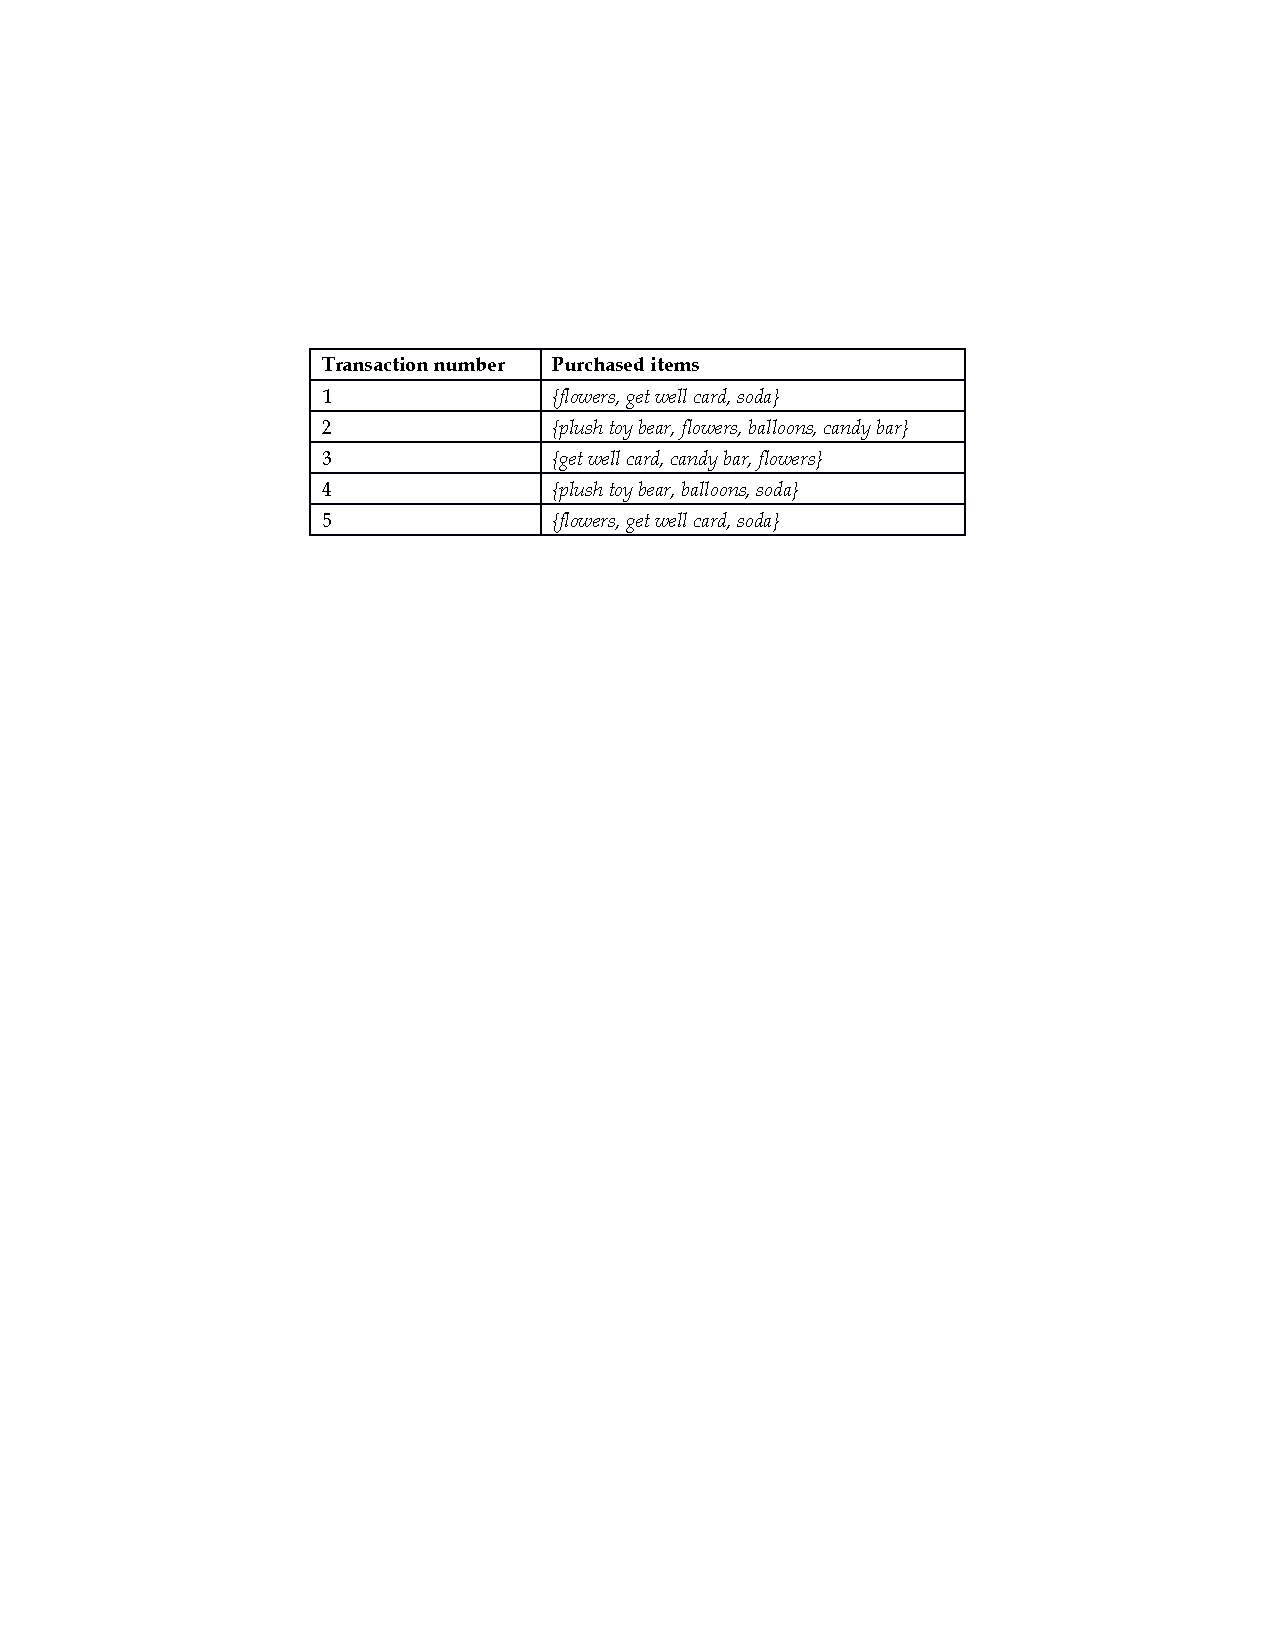
\includegraphics[scale=0.7]{table1.pdf}
\end{figure}


}

%%%%%%%%%%%%%%%%%%%%%%%%%%%%%%%%%%%%%%%%%%%%%%%

\frame{
  \frametitle{Algoritmo Apriori}


\begin{itemize}
\item  Dos patrones claros se infieren\vspace{0.3cm}

\item Quien visita a un enfermo, le compra flores y una tarjeta\vspace{0.3cm}

\item Quien visita a una nueva madre, le compra un oso y globos  \vspace{0.3cm}

\item Los patrones descritos se derivan de ciertas frecuencias \vspace{0.3cm}

\item Veremos c\'omo el algoritmo Apriori cuantifica estas frecuencias


\end{itemize}

}

%%%%%%%%%%%%%%%%%%%%%%%%%%%%%%%%%%%%%%%%%%%%%%%

\frame{
  \frametitle{Medidas de Inter\'es}


\begin{itemize}
\item  El algoritmos cuantifica qu\'e tan ``interesante'' es un itemset \vspace{0.3cm}

\item Dos medidas se usan para esto: soporte (\textit{support}) y confianza (\textit{confidence}) \vspace{0.3cm}

\item Se establencen umbrales para estas medidas y se aplica el principio Apriori \vspace{0.3cm}

\item Para reducir el n\'umero de reglas reportadas\vspace{0.3cm}

\item Veamos cada medida en detalle



\end{itemize}

}

%%%%%%%%%%%%%%%%%%%%%%%%%%%%%%%%%%%%%%%%%%%%%%%

\frame{
  \frametitle{Medida de Soporte}


\begin{itemize}
\item  El soporte de un itemset mide con qu\'e frecuencia ocurre en los datos  \vspace{0.3cm}

\item Se define como

\[
support(X) = \frac{count(X)}{N}
\]


\item donde $N$ es el n\'umero total de transacciones y $count(X)$ es el n\'umero de transacciones que contienen a $X$\vspace{0.3cm}

\item Por ejemplo, $support(\{get\ well\ card, flowers\})=3/5=0.6$\vspace{0.3cm}

\item Similarmente, $support(\{candy \ bar\})=2/5=0.4$\



\end{itemize}

}

%%%%%%%%%%%%%%%%%%%%%%%%%%%%%%%%%%%%%%%%%%%%%%%

\frame{
  \frametitle{Medida de Confianza}


\begin{itemize}
\item  La confianza de una regla mide su poder predictivo o precisi\'on   \vspace{0.3cm}

\item Se define como

\[
confidence(X\rightarrow Y)= \frac{support(X,Y)}{support(X)} 
\]

\item Es la proporci\'on de veces que ocurren $X$ y $Y$ conjuntamente, sobre eventos en los que ocurre $X$\vspace{0.3cm}

\item Si la confianza es 1, siempre que ocurre $X$, ocurre $Y$. Luego $X$ predice muy bien a $Y$





\end{itemize}

}

%%%%%%%%%%%%%%%%%%%%%%%%%%%%%%%%%%%%%%%%%%%%%%%

\frame{
  \frametitle{Medida de Confianza}


\begin{itemize}
\item     Por ejemplo,

\[
confidence(\text{flowers}\rightarrow \text{get \ well \ card})=0.6/0.8=0.75
\]

\item Con una confianza del 75\%, si alguien compra flores, compra tambi\'en la tarjeta\vspace{0.3cm}

\item Ojo: $confidence(X\rightarrow Y)\neq confidence(Y\rightarrow X)$

\[
confidence(\text{get \ well \ card} \rightarrow \text{flowers} )=0.6/0.6=1
\]

\item Con una confianza del 100\%, si alguien compra la tarjeta, compra flores tambi\'en



\end{itemize}

}

%%%%%%%%%%%%%%%%%%%%%%%%%%%%%%%%%%%%%%%%%%%%%%%

\frame{
  \frametitle{Algoritmo Apriori}


\begin{itemize}
\item  Reglas tipo  $\text{get \ well \ card} \rightarrow \text{flowers}$ son fuertes porque tienen soporte y confianza altos\vspace{0.3cm}

\item El algoritmo Apriori usa niveles m\'inimos de soporte y confianza para encontrar reglas fuertes\vspace{0.3cm}

\item Lo hace descartando reglas no interesantes\vspace{0.3cm}

\item El principio es que si $\{A,B\}$ son frecuentes, entonces \{A\} y \{B\} deben serlo tambi\'en\vspace{0.3cm}

\item Si por ej. \{A\} tiene soporte bajo (seg\'un cierto umbral), se descarta y no se considera \{A,B\}


\end{itemize}

}
%%%%%%%%%%%%%%%%%%%%%%%%%%%%%%%%%%%%%%%%%%%%%%%


\frame{
  \frametitle{Algoritmo Apriori}

El proceso de crear reglas con el algoritmo Apriori es:\vspace{0.3cm}

\begin{itemize}
\item[1.] Identificar todos los itemsets cuyos soportes superan cierto umbral m\'inimo   \vspace{0.3cm}

\item[2.] Crear reglas de estos itemsets de aquellas que cumplan cierto umbral m\'inimo de confianza




\end{itemize}

}


%%%%%%%%%%%%%%%%%%%%%%%%%%%%%%%%%%%%%%%%%%%%%%%


\frame{
  \frametitle{Medida de Confianza}


\begin{itemize}
\item  La primera fase se hace de manera iterativa\vspace{0.3cm}

\item En la iteraci\'on se eval\'uan los itemsets de tama\~no 1 \vspace{0.3cm}

\item En la 2  los de tama\~no 2. Y as\'i sucesivamente\vspace{0.3cm}

\item El resultado de cada iteraci\'on es el conjunto de itemsets cuyo soporte supera el umbral



\end{itemize}

}
%%%%%%%%%%%%%%%%%%%%%%%%%%%%%%%%%%%%%%%%%%%%%%%

\frame{
  \frametitle{Ejemplo}


\begin{itemize}

\item Supongamos cuatro items: A, B, C, D \vspace{0.3cm}

\item Solo A, B, C cumplen con el soporte m\'inimo; D se descarta en la primera iteraci\'on\vspace{0.3cm}

\item En la segunda solo se eval\'uan \{A,B\}, \{A,C\} y \{B,C\}\vspace{0.3cm}

\item Supongamos que solo \{A,B\} y \{A,C\} son frecuentes. Se descarta \{B,C\}\vspace{0.3cm}

\item Luego, el algoritmo se detiene y no debe evaluar \{A, B, C\}





\end{itemize}

}
%%%%%%%%%%%%%%%%%%%%%%%%%%%%%%%%%%%%%%%%%%%%%%%

\frame{
  \frametitle{Ejemplo}


\begin{itemize}

\item Luego de esto arranca la segunda fase del algortimo \vspace{0.3cm}

\item Se forman las reglas de asociaci\'on\vspace{0.3cm}

\item Por ejemplo, $A\rightarrow B$ o $B\rightarrow A$\vspace{0.3cm}

\item Sobreviven las que superen el umbral de la medida de confianza\vspace{0.3cm}

\item Se interpretan las reglas finales







\end{itemize}

}
%%%%%%%%%%%%%%%%%%%%%%%%%%%%%%%%%%%%%%%%%%%%%%%

\frame{
  \frametitle{Reglas de Asociaci\'on }


\begin{itemize}

\item ?`C\'omo medir la importancia de una regla? \vspace{0.3cm}

\item El soporte y la confianza cumplen este prop\'osito\vspace{0.3cm}

\item Pero hay otra medida: el lift:

\[
lift(X\rightarrow Y)=\frac{confidence(X\rightarrow Y)}{support(Y)}
\]







\end{itemize}

}
%%%%%%%%%%%%%%%%%%%%%%%%%%%%%%%%%%%%%%%%%%%%%%%

\frame{
  \frametitle{Reglas de Asociaci\'on }


\begin{itemize}

\item El lift mide qu\'e tanto es m\'as probable que se compre Y dado que se compra X, en relaci\'on a su tasa t\'ipica de compra \vspace{0.3cm}

\item Luego mide qu\'e tanto ganamos sobre la probabilidad de compra de Y al saber que X se compra\vspace{0.3cm}

\item Si lift es mayor que 1, sabemos que es m\'as probable que se compre Y cuando se compra X respecto a la tasa t\'ipica\vspace{0.3cm}

\item Reglas con lift alto tienen mayor importancia







\end{itemize}

}
%%%%%%%%%%%%%%%%%%%%%%%%%%%%%%%%%%%%%%%%%%%%%%%


\frame{
  \frametitle{Reglas de Asociaci\'on }

Conviene clasificar a las reglas finales en una de tres categor�as\vspace{0.3cm}

\begin{itemize}

\item[1.] Accionables \vspace{0.3cm}

\item[2.] Triviales \vspace{0.3cm}

\item[3.] Inexplicables \vspace{0.3cm}

\end{itemize}

El objetivo es encontrar reglas accionables

}
%%%%%%%%%%%%%%%%%%%%%%%%%%%%%%%%%%%%%%%%%%%%%%%


\end{document}


